\newcommand{\kcas}{%
  \kappa%
}

\newcommand{\similar}{%
  \approx%
}
\newcommand{\nonsimilar}{%
  \not\approx
}

\newcommand{\view}{%
  \mathcal{V}%
}
\newcommand{\viewTwo}{%
  \mathcal{W}%
}
\newcommand{\viewJoin}[2]{%
  #1 \sqcup #2%
}

\newcommand{\iKcasPointsto}{%
  \rightarrowtail%
}
\newcommand{\iView}[1]{%
  \sqsupseteq #1%
}

\newcommand{\colorLoc}{blue}
\newcommand{\colorBefore}{red}
\newcommand{\colorAfter}{Green}
\newcommand{\colorReadOnly}{cyan}
\newcommand{\colorResult}{orange}
\newcommand{\colorView}{brown}

% ---------------------------------------------------------

\section{Specimen: \Kcas (ongoing work)}

\begin{frame}[fragile]{\Kcas: software transactional memory for \OCaml}
\Large
\begin{minted}{ocaml}
let a = Loc.make 10 in
let b = Loc.make 52 in
let x = Loc.make 0 in

let tx ~xt =
  let a = Xt.get ~xt a in
  let b = Xt.get ~xt b in
  Xt.set ~xt x (b - a)
in

Xt.commit { tx }
\end{minted}
\end{frame}

\begin{frame}[fragile]{\Kcas: software transactional memory for \OCaml}
\centering
\Large
\begin{minted}{ocaml}
type ('k, 'v) cache =
  { space: int Loc.t; 
    table: ('k, 'k Dllist.Xt.node * 'v) Hashtbl.Xt.t;
    order: 'k Dllist.Xt.t;
  }
\end{minted}
\end{frame}

\begin{frame}[fragile]{MCAS}
\LARGE
\begin{minted}{ocaml}
let a = Loc.make 10 in
let b = Loc.make 52 in
let x = Loc.make 0 in
\end{minted}
\vfill
\begin{minipage}{0.5\textwidth}
  \begin{minted}{ocaml}
let a = Xt.get ~xt a in
let b = Xt.get ~xt b in
Xt.set ~xt x (b - a)
  \end{minted}
\end{minipage}
\hfill
\begin{minipage}{0.4\textwidth}
  \begin{minted}{ocaml}
CAS (a, 10, 10)
CAS (b, 52, 52)
CAS (x, 0, 42)
  \end{minted}
\end{minipage}
\end{frame}

\begin{frame}{MCAS specification}
\centering
\large
\[
  \iAspec{
    \displaystyle\iBigSep_{\textcolor{\colorLoc}{\loc} \in \textcolor{\colorLoc}{\loc s}} \mathrm{loc \mathhyphen inv}\ \textcolor{\colorLoc}{\loc}\ \inv
  }{
    \mathit{vs}
  }{
    \displaystyle\iBigSep_{\textcolor{\colorLoc}{\loc}, v \in \textcolor{\colorLoc}{\loc s}, \mathit{vs}} \textcolor{\colorLoc}{\loc} \iKcasPointsto v
  }{
    \texttt{mcas}\ \textcolor{\colorLoc}{\loc s}\ \textcolor{\colorBefore}{\mathit{befores}}\ \textcolor{\colorAfter}{\mathit{afters}},\ \uparrow\inv
  }{
    \textcolor{\colorResult}{b}
  }{
    \begin{array}{l}
        \textbf{if}\ \textcolor{\colorResult}{b}\ \textbf{then}\ 
        \mathit{vs} = \textcolor{\colorBefore}{\mathit{befores}} \iSep
        \displaystyle\iBigSep_{\textcolor{\colorLoc}{\loc}, v \in \textcolor{\colorLoc}{\loc s}, \textcolor{\colorAfter}{\mathit{afters}}} \textcolor{\colorLoc}{\loc} \iKcasPointsto v
      \\
        \textbf{else}\ 
        \exists i \ldotp
        \mathit{vs}_i \neq \textcolor{\colorBefore}{\mathit{befores}}_i
        \displaystyle\iBigSep_{\textcolor{\colorLoc}{\loc}, v \in \textcolor{\colorLoc}{\loc s}, \mathit{vs}} \textcolor{\colorLoc}{\loc} \iKcasPointsto v
    \end{array}
  }{
    \textcolor{\colorResult}{b}
  }{
    \iTrue
  }
\]
\end{frame}

\begin{frame}{MCAS specification: taking physical equality seriously}
\centering
\large
\[
  \iAspec{
    \displaystyle\iBigSep_{\textcolor{\colorLoc}{\loc} \in \textcolor{\colorLoc}{\loc s}} \mathrm{loc \mathhyphen inv}\ \textcolor{\colorLoc}{\loc}\ \inv
  }{
    \mathit{vs}
  }{
    \displaystyle\iBigSep_{\textcolor{\colorLoc}{\loc}, v \in \textcolor{\colorLoc}{\loc s}, \mathit{vs}} \textcolor{\colorLoc}{\loc} \iKcasPointsto v
  }{
    \texttt{mcas}\ \textcolor{\colorLoc}{\loc s}\ \textcolor{\colorBefore}{\mathit{befores}}\ \textcolor{\colorAfter}{\mathit{afters}},\ \uparrow\inv
  }{
    \textcolor{\colorResult}{b}
  }{
    \begin{array}{l}
        \textbf{if}\ \textcolor{\colorResult}{b}\ \textbf{then}\ 
        \mathit{vs} \similar \textcolor{\colorBefore}{\mathit{befores}} \iSep
        \displaystyle\iBigSep_{\textcolor{\colorLoc}{\loc}, v \in \textcolor{\colorLoc}{\loc s}, \textcolor{\colorAfter}{\mathit{afters}}} \textcolor{\colorLoc}{\loc} \iKcasPointsto v
      \\
        \textbf{else}\ 
        \exists i \ldotp
        \mathit{vs}_i \nonsimilar \textcolor{\colorBefore}{\mathit{befores}}_i
        \displaystyle\iBigSep_{\textcolor{\colorLoc}{\loc}, v \in \textcolor{\colorLoc}{\loc s}, \mathit{vs}} \textcolor{\colorLoc}{\loc} \iKcasPointsto v
    \end{array}
  }{
    \textcolor{\colorResult}{b}
  }{
    \iTrue
  }
\]
\end{frame}

\begin{frame}{MCAS specification: read-only locations}
\centering
\large
\[
  \iAspec{
    \displaystyle\iBigSep_{\textcolor{\colorReadOnly}{\loc} \in \textcolor{\colorReadOnly}{\loc s}} \mathrm{loc \mathhyphen inv}\ \textcolor{\colorReadOnly}{\loc}\ \inv \iSep
    \displaystyle\iBigSep_{\textcolor{\colorLoc}{\loc} \in \textcolor{\colorLoc}{\loc s}} \mathrm{loc \mathhyphen inv}\ \textcolor{\colorLoc}{\loc}\ \inv
  }{
    \mathit{ws}, \mathit{vs}
  }{
    \displaystyle\iBigSep_{\textcolor{\colorReadOnly}{\loc}, v \in \textcolor{\colorReadOnly}{\loc s}, \mathit{ws}} \textcolor{\colorReadOnly}{\loc} \iKcasPointsto v \iSep
    \displaystyle\iBigSep_{\textcolor{\colorLoc}{\loc}, v \in \textcolor{\colorLoc}{\loc s}, \mathit{vs}} \textcolor{\colorLoc}{\loc} \iKcasPointsto v
  }{
    \texttt{mcas}\ \textcolor{\colorReadOnly}{\loc s}\ \textcolor{\colorLoc}{\loc s}\ \textcolor{\colorBefore}{\mathit{befores}}\ \textcolor{\colorAfter}{\mathit{afters}},\ \uparrow\inv
  }{
    \textcolor{\colorResult}{b}
  }{
    \displaystyle\iBigSep_{\textcolor{\colorReadOnly}{\loc}, v \in \textcolor{\colorReadOnly}{\loc s}, \mathit{ws}} \textcolor{\colorReadOnly}{\loc} \iKcasPointsto v \iSep
    \begin{array}{l}
        \textbf{if}\ \textcolor{\colorResult}{b}\ \textbf{then}\ 
        \mathit{vs} \similar \textcolor{\colorBefore}{\mathit{befores}} \iSep
        \displaystyle\iBigSep_{\textcolor{\colorLoc}{\loc}, v \in \textcolor{\colorLoc}{\loc s}, \textcolor{\colorAfter}{\mathit{afters}}} \textcolor{\colorLoc}{\loc} \iKcasPointsto v
      \\
        \textbf{else}\ 
        \displaystyle\iBigSep_{\textcolor{\colorLoc}{\loc}, v \in \textcolor{\colorLoc}{\loc s}, \mathit{vs}} \textcolor{\colorLoc}{\loc} \iKcasPointsto v
    \end{array}
  }{
    \textcolor{\colorResult}{b}
  }{
    \iTrue
  }
\]
\end{frame}

\begin{frame}{MCAS specification: relaxed memory}
\centering
\large
\[
  \iAspec{
    \iView{\textcolor{\colorView}{\viewTwo}} \iSep
    \displaystyle\iBigSep_{\textcolor{\colorLoc}{\loc} \in \textcolor{\colorLoc}{\loc s}} \mathrm{loc \mathhyphen inv}\ \textcolor{\colorLoc}{\loc}\ \inv
  }{
    \mathit{vs}, \textcolor{\colorView}{\view s}
  }{
    \displaystyle\iBigSep_{\textcolor{\colorLoc}{\loc}, v, \textcolor{\colorView}{\view} \in \textcolor{\colorLoc}{\loc s}, \mathit{vs}, \textcolor{\colorView}{\view s}} \textcolor{\colorLoc}{\loc} \iKcasPointsto (v, \textcolor{\colorView}{\view})
  }{
    \texttt{mcas}\ \textcolor{\colorLoc}{\loc s}\ \textcolor{\colorBefore}{\mathit{befores}}\ \textcolor{\colorAfter}{\mathit{afters}},\ \uparrow\inv
  }{
    \textcolor{\colorResult}{b}
  }{
    \begin{array}{l}
        \textbf{if}\ \textcolor{\colorResult}{b}\ \textbf{then}\ 
        \mathit{vs} \similar \textcolor{\colorBefore}{\mathit{befores}} \iSep
        \displaystyle\iBigSep_{\textcolor{\colorLoc}{\loc}, v, \textcolor{\colorView}{\view} \in \textcolor{\colorLoc}{\loc s}, \textcolor{\colorAfter}{\mathit{afters}}, \textcolor{\colorView}{\view s}} \textcolor{\colorLoc}{\loc} \iKcasPointsto (v, \viewJoin{\textcolor{\colorView}{\view}}{\textcolor{\colorView}{\viewTwo}})
      \\
        \textbf{else}\ 
        \exists i \ldotp
        \mathit{vs}_i \nonsimilar \textcolor{\colorBefore}{\mathit{befores}}_i
        \displaystyle\iBigSep_{\textcolor{\colorLoc}{\loc}, v, \textcolor{\colorView}{\view} \in \textcolor{\colorLoc}{\loc s}, \mathit{vs}, \textcolor{\colorView}{\view s}} \textcolor{\colorLoc}{\loc} \iKcasPointsto (v, \textcolor{\colorView}{\view})
    \end{array}
  }{
    \textcolor{\colorResult}{b}
  }{
    \displaystyle\iBigSep_{\textcolor{\colorView}{\view} \in \textcolor{\colorView}{\view s}} \iView{\textcolor{\colorView}{\view}}
  }
\]
\end{frame}

\begin{frame}{MCAS algorithm: Harris, Fraser \& Pratt (2002)}
\centering
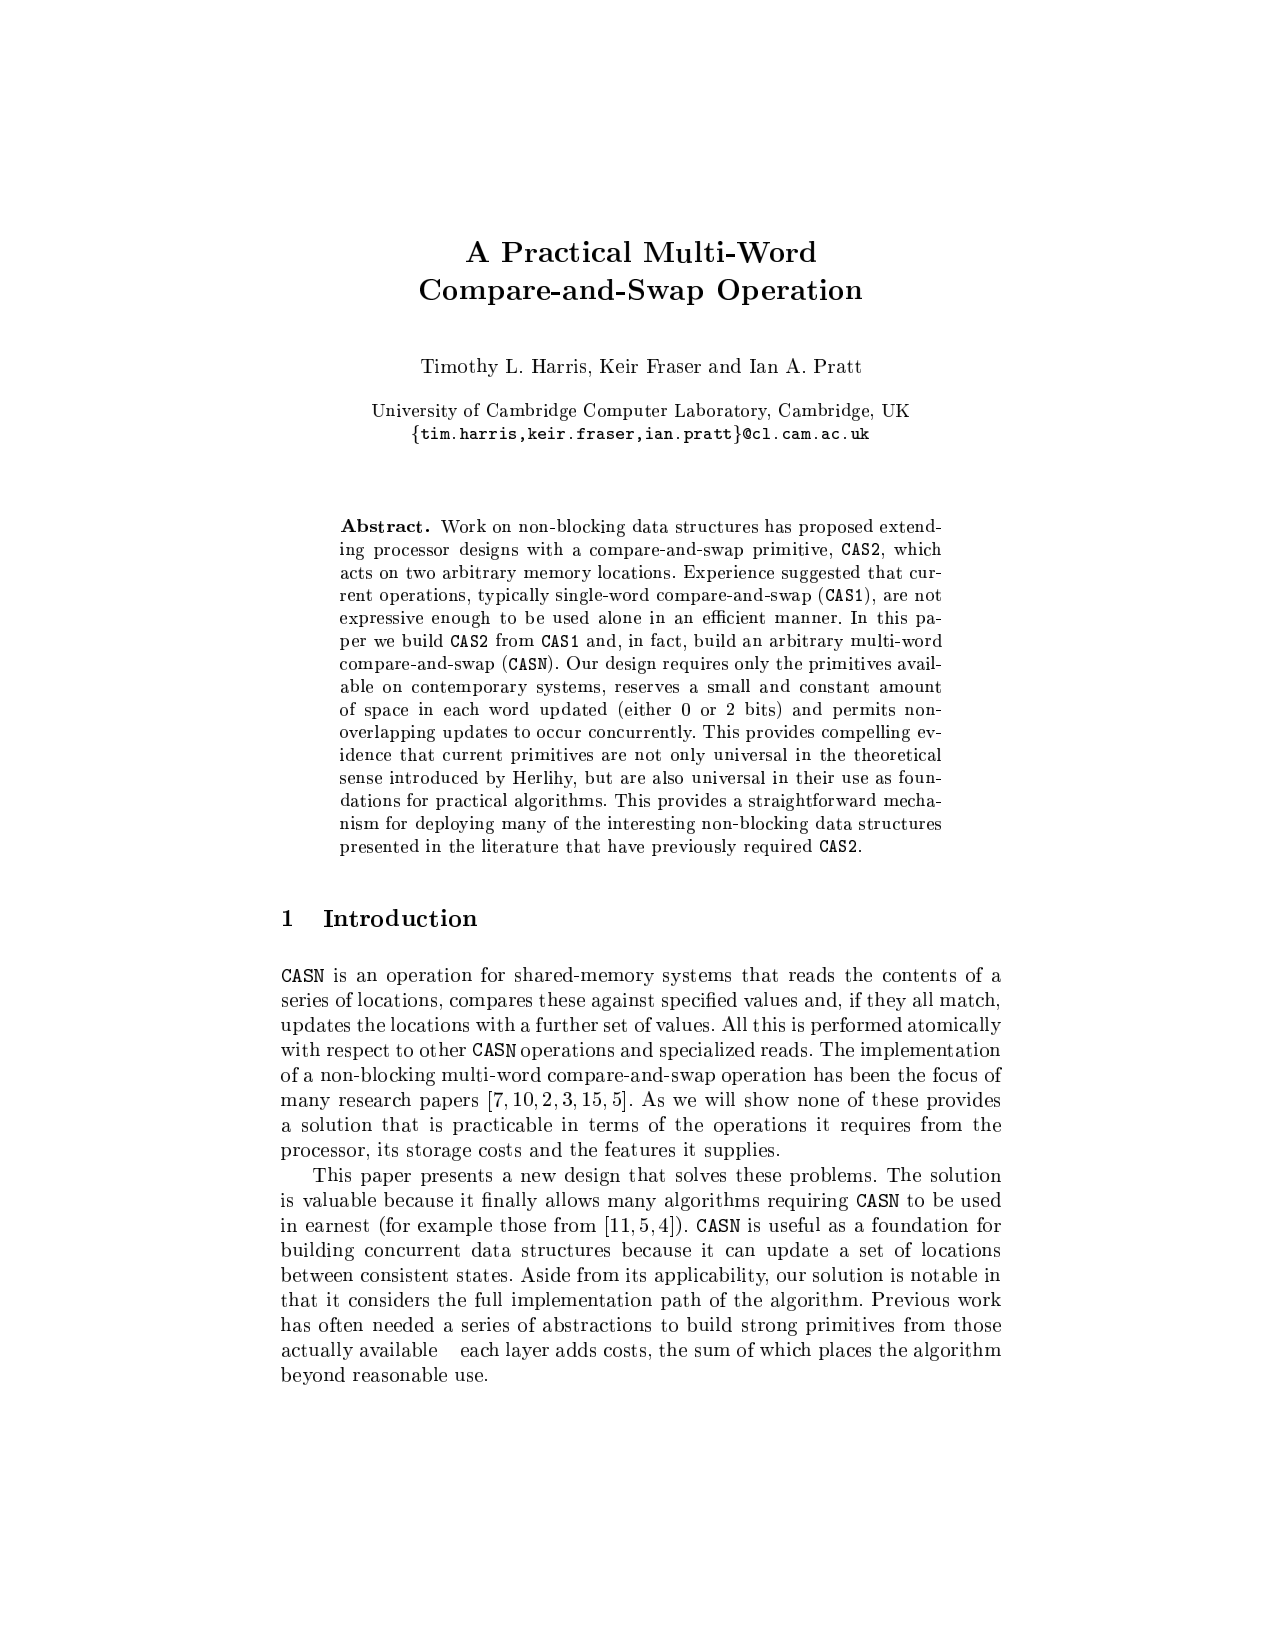
\includegraphics[scale=0.5]{images/harris_fraser_pratt_2002.pdf}
\end{frame}

\begin{frame}{Verified RDCSS by Jung \etal}
\centering
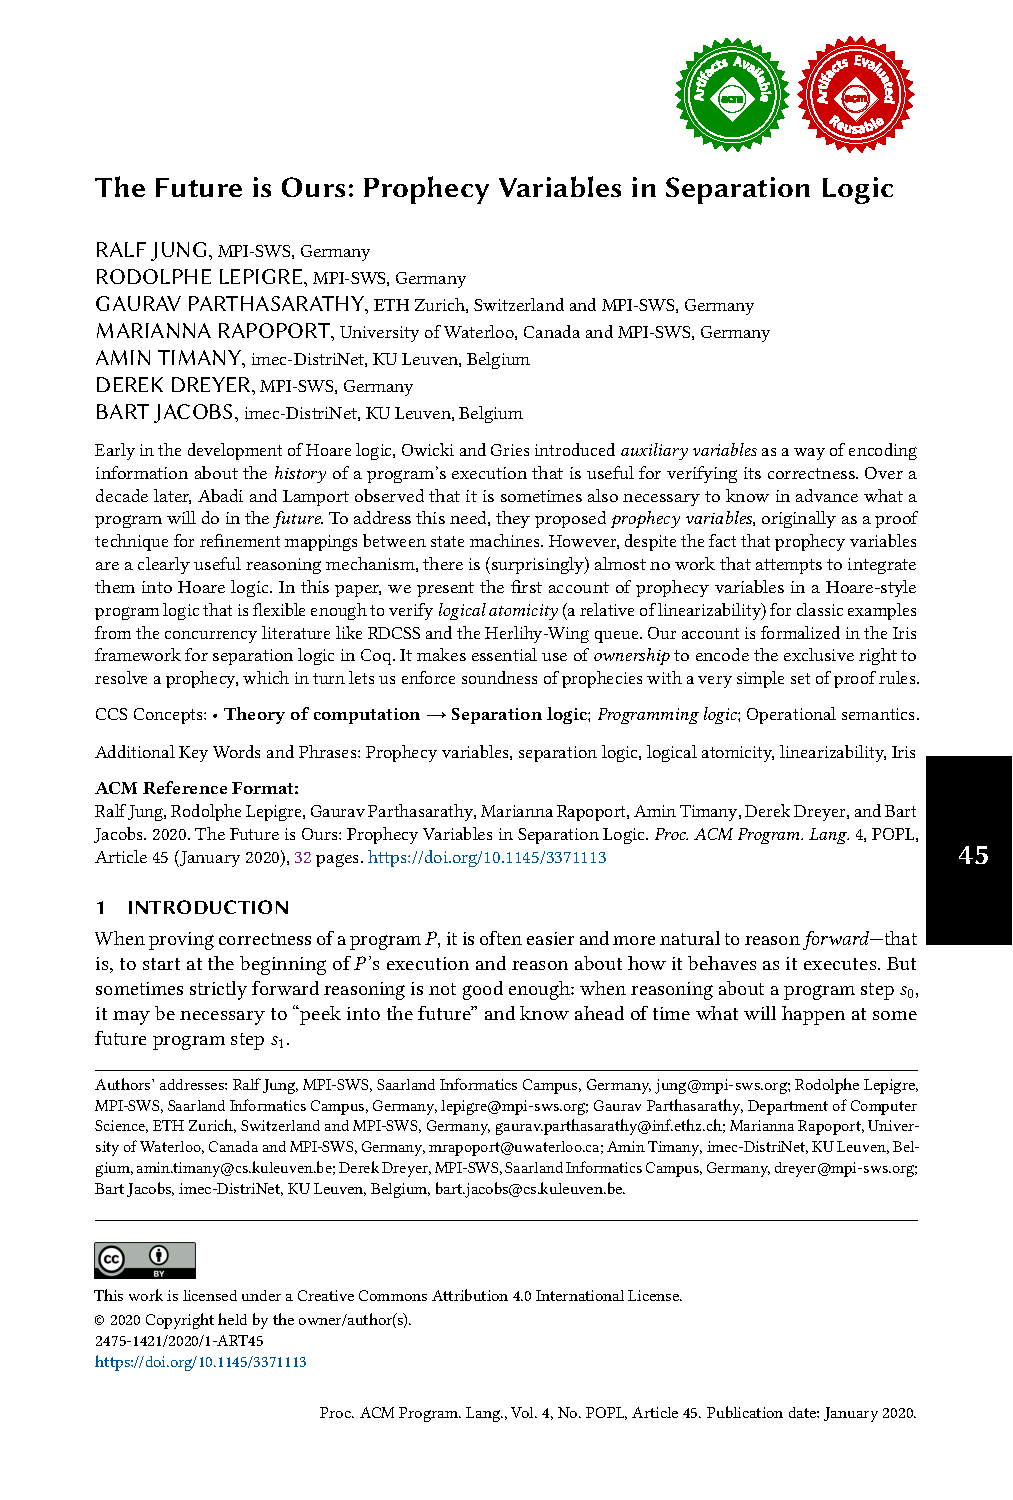
\includegraphics[scale=0.5]{images/jung_lepigre_parthasarathy_2020.pdf}
\end{frame}

\begin{frame}{MCAS algorithm: Guerraoui, Kogan, Marathe \& Zablotchi (2020)}
\centering
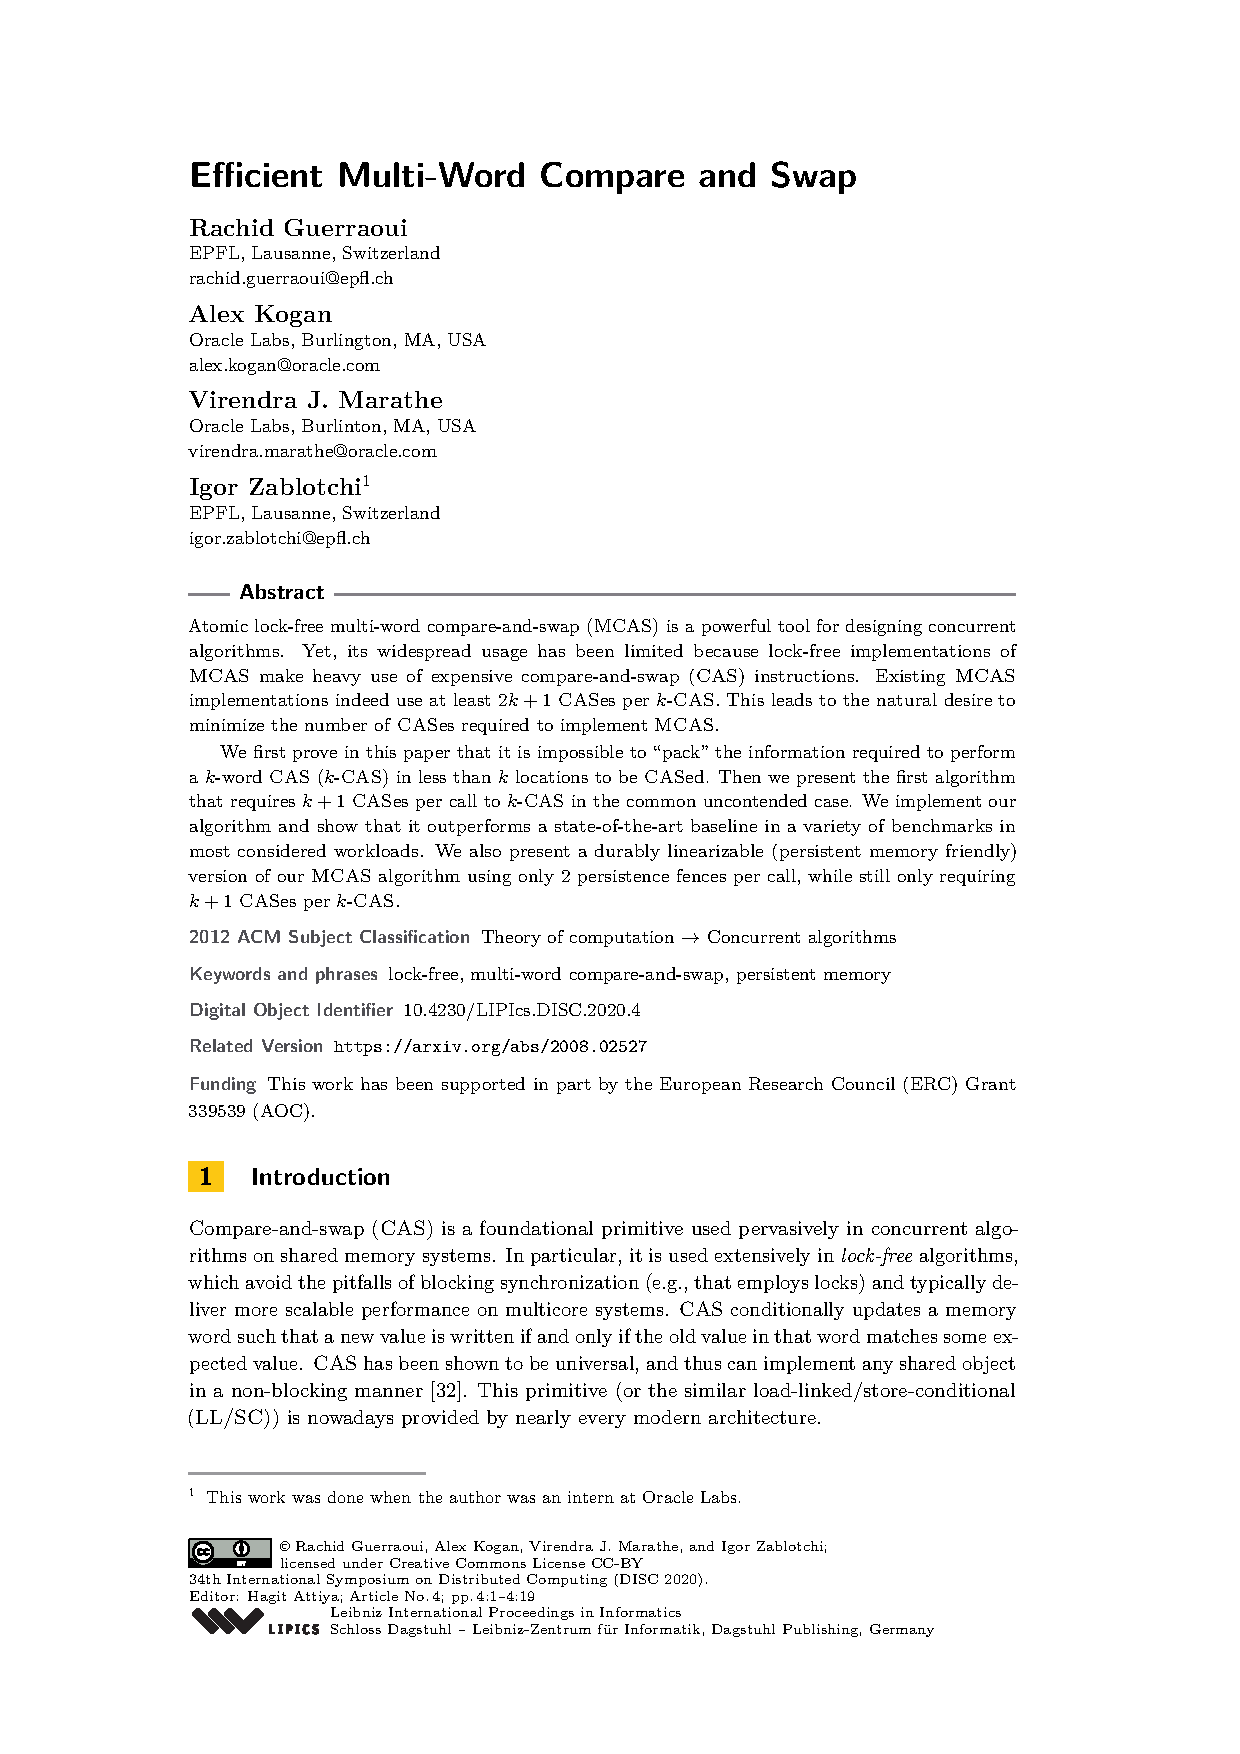
\includegraphics[scale=0.5]{images/guerraoui_kogan_marathe_zablotchi_2020.pdf}
\end{frame}

\begin{frame}{MCAS location}
\centering
\Large
\[
  \loc \iKcasPointsto v_1\ \text{or}\ v_2
\]
\vfill
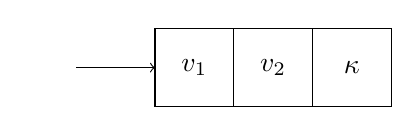
\begin{tikzpicture}[yscale=-1]
  \node at (0.5,0.5) {$\loc$} ;
  \draw [->] (1,0.5) -- ++(1,0) ;
  \draw (2,0) grid ++(3,1) ;
  \node at (2.5,0.5) {$v_1$} ;
  \node at (3.5,0.5) {$v_2$} ;
  \node at (4.5,0.5) {$\kappa$} ;
\end{tikzpicture}
\end{frame}

\begin{frame}{Finished MCAS}
\centering
\Large
\begin{minipage}[t][0.6\textheight]{0.48\textwidth}
  \[
    \loc \iKcasPointsto v_1
  \]
  \vfill
  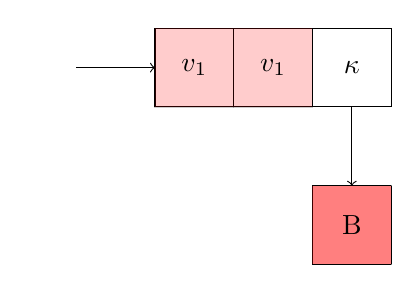
\begin{tikzpicture}[yscale=-1]
    \node at (0.5,0.5) {$\loc$} ;
    \draw [->] (1,0.5) -- ++(1,0) ;
    \draw (2,0) grid ++(3,1) ;
    \draw [fill=red, opacity=0.2] (2,0) rectangle ++(1,1) ;
    \node at (2.5,0.5) {$v_1$} ;
    \draw [fill=red, opacity=0.2] (3,0) rectangle ++(1,1) ;
    \node at (3.5,0.5) {$v_1$} ;
    \node at (4.5,0.5) {$\kappa$} ;
    \draw [->] (4.5,1) -- ++(0,1) ;
    \draw (4,2) grid ++(1,1) ;
    \draw [fill=red, opacity=0.5] (4,2) rectangle ++(1,1) ;
    \node at (4.5,2.5) {B} ;
  \end{tikzpicture}
\end{minipage}
\begin{minipage}[t][0.6\textheight]{0.48\textwidth}
  \[
    \loc \iKcasPointsto v_2
  \]
  \vfill
  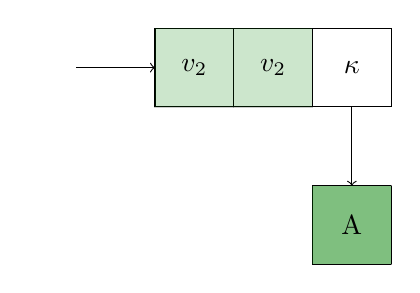
\begin{tikzpicture}[yscale=-1]
    \node at (0.5,0.5) {$\loc$} ;
    \draw [->] (1,0.5) -- ++(1,0) ;
    \draw (2,0) grid ++(3,1) ;
    \draw [fill=Green, opacity=0.2] (2,0) rectangle ++(1,1) ;
    \node at (2.5,0.5) {$v_2$} ;
    \draw [fill=Green, opacity=0.2] (3,0) rectangle ++(1,1) ;
    \node at (3.5,0.5) {$v_2$} ;
    \node at (4.5,0.5) {$\kappa$} ;
    \draw [->] (4.5,1) -- ++(0,1) ;
    \draw (4,2) grid ++(1,1) ;
    \draw [fill=Green, opacity=0.5] (4,2) rectangle ++(1,1) ;
    \node at (4.5,2.5) {A} ;
  \end{tikzpicture}
\end{minipage}
\end{frame}

\begin{frame}{Undetermined MCAS}
\centering
\Large
\[
  \loc \iKcasPointsto v_1
\]
\vfill
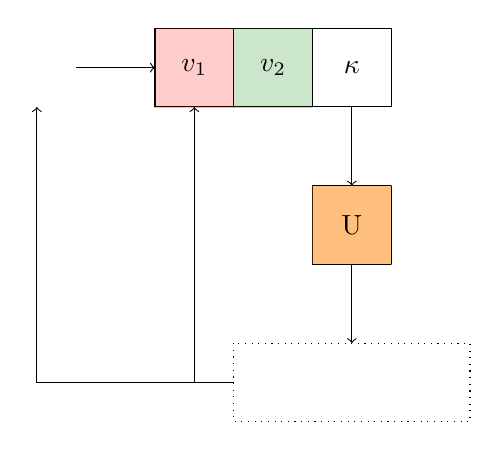
\begin{tikzpicture}[yscale=-1]
  \node at (0.5,0.5) {$\loc$} ;
  \draw [->] (1,0.5) -- ++(1,0) ;
  \draw (2,0) grid ++(3,1) ;
  \draw [fill=red, opacity=0.2] (2,0) rectangle ++(1,1) ;
  \node at (2.5,0.5) {$v_1$} ;
  \draw [fill=Green, opacity=0.2] (3,0) rectangle ++(1,1) ;
  \node at (3.5,0.5) {$v_2$} ;
  \node at (4.5,0.5) {$\kappa$} ;
  \draw [->] (4.5,1) -- ++(0,1) ;
  \draw (4,2) grid ++(1,1) ;
  \draw [fill=orange, opacity=0.5] (4,2) rectangle ++(1,1) ;
  \node at (4.5,2.5) {U} ;
  \draw [->] (4.5,3) -- ++(0,1) ;
  \draw [dotted] (3,4) rectangle ++(3,1) ;
  \draw [->] (3,4.5) -| (0.5,1) ;
  \draw [->] (3,4.5) -| (2.5,1) ;
\end{tikzpicture}
\end{frame}

\begin{frame}{MCAS algorithm}
\centering
\large
\begin{tikzpicture}[yscale=-1]
  \node at (0.5,0.5) {$\loc_1$} ;
  
  \draw (2,0) grid ++(3,1) ;
  \draw [fill=Green, opacity=0.2] (2,0) rectangle ++(1,1) ;
  \node at (2.5,0.5) {1} ;
  \draw [fill=Green, opacity=0.2] (3,0) rectangle ++(1,1) ;
  \node at (3.5,0.5) {1} ;
  \node at (4.5,0.5) {$\kappa_1$} ;
  \draw [->] (4.5,0) -- ++(0,-1) ;
  \draw (4,-2) grid ++(1,1) ;
  \draw [fill=Green, opacity=0.5] (4,-2) rectangle ++(1,1) ;
  \node at (4.5,-1.5) {A} ;
  
  \node at (7.5,0.5) {$\loc_2$} ;
  
  \draw (9,0) grid ++(3,1) ;
  \draw [fill=Green, opacity=0.2] (9,0) rectangle ++(1,1) ;
  \node at (9.5,0.5) {3} ;
  \draw [fill=Green, opacity=0.2] (10,0) rectangle ++(1,1) ;
  \node at (10.5,0.5) {3} ;
  \node at (11.5,0.5) {$\kappa_2$} ;
  \draw [->] (11.5,0) -- ++(0,-1) ;
  \draw (11,-2) grid ++(1,1) ;
  \draw [fill=Green, opacity=0.5] (11,-2) rectangle ++(1,1) ;
  \node at (11.5,-1.5) {A} ;
  
  \draw (2,2) grid ++(3,1) ;
  \only<1-4,7->{
    \draw [fill=red, opacity=0.2] (2,2) rectangle ++(1,1) ;
    \node at (2.5,2.5) {1} ;
  }
  \only<5-6>{
    \draw [fill=Green, opacity=0.2] (2,2) rectangle ++(1,1) ;
    \node at (2.5,2.5) {2} ;
  }
  \only<1-8>{
    \draw [fill=Green, opacity=0.2] (3,2) rectangle ++(1,1) ;
    \node at (3.5,2.5) {2} ;
  }
  \only<9->{
    \draw [fill=red, opacity=0.2] (3,2) rectangle ++(1,1) ;
    \node at (3.5,2.5) {1} ;
  }
  \node at (4.5,2.5) {$\kappa$} ;
  
  \draw (9,2) grid ++(3,1) ;
  \only<1-5>{
    \draw [fill=red, opacity=0.2] (9,2) rectangle ++(1,1) ;
    \node at (9.5,2.5) {3} ;
  }
  \only<6>{
    \draw [fill=Green, opacity=0.2] (9,2) rectangle ++(1,1) ;
    \node at (9.5,2.5) {2} ;
  }
  \only<7->{
    \draw [fill=red, opacity=0.2] (9,2) rectangle ++(1,1) ;
    \node at (9.5,2.5) {0} ;
  }
  \only<1-9>{
    \draw [fill=Green, opacity=0.2] (10,2) rectangle ++(1,1) ;
    \node at (10.5,2.5) {2} ;
  }
  \only<10->{
    \draw [fill=red, opacity=0.2] (10,2) rectangle ++(1,1) ;
    \node at (10.5,2.5) {0} ;
  }
  \node at (11.5,2.5) {$\kappa$} ;
  
  \only<1-3,7>{
    \draw [fill=orange, opacity=0.5] (7,4) rectangle ++(1,1) ;
    \node at (7.5,4.5) {U} ;
  }
  \only<4-6>{
    \draw [fill=Green, opacity=0.5] (7,4) rectangle ++(1,1) ;
    \node at (7.5,4.5) {A} ;
  }
  \only<8->{
    \draw [fill=red, opacity=0.5] (7,4) rectangle ++(1,1) ;
    \node at (7.5,4.5) {B} ;
  }
  
  \draw [->] (4.5,3) |- (7,4.5) ;
  \draw [->] (11.5,3) |- (8,4.5) ;
  
  \only<1>{
    \draw [->] (1,0.5) -- ++(1,0) ;
  }
  \only<2,7>{
    \draw [->, orange] (0.5,1) |- (2,2.5) ;
  }
  \only<3-6,8->{
    \draw [->] (0.5,1) |- (2,2.5) ;
  }
  
  \only<1-2,7->{
    \draw [->] (8,0.5) -- ++(1,0) ;
  }
  \only<3>{
    \draw [->, orange] (7.5,1) |- (9,2.5) ;
  }
  \only<4-6>{
    \draw [->] (7.5,1) |- (9,2.5) ;
  }
\end{tikzpicture}
\end{frame}
